\documentclass[a4paper,10pt,ngerman]{scrartcl}
\usepackage{babel}
\usepackage[T1]{fontenc}
\usepackage[utf8x]{inputenc}
\usepackage[a4paper,margin=2.5cm,footskip=0.5cm]{geometry}

% Die nächsten drei Felder bitte anpassen:
\newcommand{\Aufgabe}{Aufgabe 1: \LaTeX-Dokument} % Aufgabennummer und Aufgabennamen angeben
\newcommand{\TeilnahmeId}{?????}                  % Teilnahme-ID angeben
\newcommand{\Name}{Vor- und Nachname}             % Name des Bearbeiter / der Bearbeiterin dieser Aufgabe angeben

% Kopf- und Fußzeilen
\usepackage{scrlayer-scrpage, lastpage}
\setkomafont{pageheadfoot}{\large\textrm}
\lohead{\Aufgabe}
\rohead{Teilnahme-ID: \TeilnahmeId}
\cfoot*{\thepage{}/\pageref{LastPage}}

% Position des Titels
\usepackage{titling}
\setlength{\droptitle}{-1.0cm}

% Für mathematische Befehle und Symbole
\usepackage{amsmath}
\usepackage{amssymb}

% Für Bilder
\usepackage{graphicx}

% Für Algorithmen
\usepackage{algpseudocode}

\usepackage{tabularx}
\usepackage{booktabs}

% Für Quelltext
\usepackage{listings}
\usepackage{color}
\definecolor{mygreen}{rgb}{0,0.6,0}
\definecolor{mygray}{rgb}{0.5,0.5,0.5}
\definecolor{mymauve}{rgb}{0.58,0,0.82}
\lstset{
  keywordstyle=\color{blue},commentstyle=\color{mygreen},
  stringstyle=\color{mymauve},rulecolor=\color{black},
  basicstyle=\footnotesize\ttfamily,numberstyle=\tiny\color{mygray},
  captionpos=b, % sets the caption-position to bottom
  keepspaces=true, % keeps spaces in text
  numbers=left, numbersep=5pt, showspaces=false,showstringspaces=true,
  showtabs=false, stepnumber=2, tabsize=2, title=\lstname
}
\lstdefinelanguage{JavaScript}{ % JavaScript ist als einzige Sprache noch nicht vordefiniert
  keywords={break, case, catch, continue, debugger, default, delete, do, else, finally, for, function, if, in, instanceof, new, return, switch, this, throw, try, typeof, var, void, while, with},
  morecomment=[l]{//},
  morecomment=[s]{/*}{*/},
  morestring=[b]',
  morestring=[b]",
  sensitive=true
}

% Diese beiden Pakete müssen zuletzt geladen werden
%\usepackage{hyperref} % Anklickbare Links im Dokument
\usepackage{cleveref}

% Daten für die Titelseite
\title{\textbf{\Huge\Aufgabe}}
\author{\LARGE Teilnahme-ID: \LARGE \TeilnahmeId \\\\
  \LARGE Bearbeiter/-in dieser Aufgabe: \\
  \LARGE \Name\\\\}
\date{\LARGE\today}

\begin{document}

\maketitle
\tableofcontents

\vspace{0.5cm}

\section{Lösungsidee}
\subsection{Notation}
Die Menge der möglichen Stapel der Höhe $n$ wird mit $\mathsf{P}_n$ bezeichnet.
Die Möglichen Pfannkuchen-Wende-und-Ess-Operationen für einem Stapel mit $n$
Pfannkuchen wird mit $\mathsf{W}_n$ bezeichnet. Die Menge der möglichen
Umkehroperationen für solch einen Stapel wird mit $\mathsf{W}^{-1}_n$
bezeichnet. Wenn der Stapel $S \in \mathsf{P}_n$ durch die Operation $w \in
  \mathsf{W}_n$ verändert wird, so wird der neue Stapel $S' = w S$ bezeichnet.
Operationen assoziieren nach rechts, d.h. $w_1 w_2 S = w_1 (w_2 S)$. Die
Funktionen $A$ und $P$ werden aus der Aufgabenstellung übernommen. Wird ein
Stapel im Text dargestellt, dann steht der erste Pfannkuchen für den obersten,
der zweite für den zweitobersten und so weiter. Pfannkuchenstapel werden
entweder in Klammern durch Kommas getrennt (z.B. $(2,7,1,8)$) oder als nicht
getrennte Ziffern dargestellt (z.B. $2718$). Bei der zweiten Notation können
Pfannkuchen dann maximal die Breite 9 haben, um die Eindeutigkeit der
Darstellung zu gewährleisten.
\subsection{Sortieren}
\begin{figure}[t]
  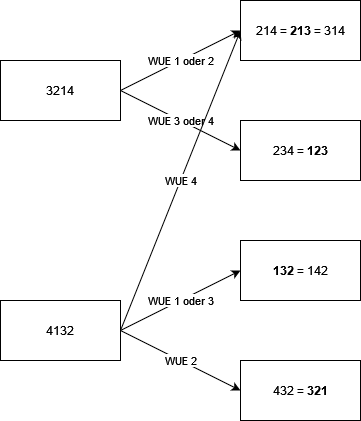
\includegraphics[scale=0.5]{pancakegraph}
  \centering
  \caption{Ausschnitt aus dem Graph der Pfannkuchenstapel. Die Kanten sind beschriftet mit der zugehörigen Operation.}
\end{figure}
Die möglichen Stapel können in einem gerichteten Graphen dargestellt werden (Siehe Abbildung 1). Die Knoten des Graphen
sind die Stapel, die Kanten sind die Operationen. Die Kanten sind gerichtet, denn eine PWUE-Operation
wandelt einen Stapel in einen anderen um. Die Identität eines Stapels wird durch die Reihenfolge der Pfannkuchen bestimmt,
nicht deren genauen Größen. Das heißt, dass zum Beispiel die Stapel $(10,12,3)$ und $(2,3,1)$ gleich sind, denn die Elemente haben die gleiche
Reihenfolge. Das hängt damit zusammen, dass der Zielstapel nur durch seine aufsteigende Reihenfolge definiert ist. Equivalente Stapel können
in eine kanonische Form gebracht werden, in dem die kleinste Größe durch 1, die zweitkleinste durch 2 und so weiter ersetzt werden. Dadurch ist
$(2,3,1)$ in kanonischer Form.
\\
Um die Operationen zu bestimmen, die einen Stapel optimal sortieren, muss
ein kürzester Pfad im Graphen vom Stapel zu einem sortierten Stapel gefunden werden. Dafür lässt sich
Dijkstra's Algorithmus \cite{dijkstra_1959} verwenden.
\begin{algorithmic}
  \Procedure{Dijkstra's Algorithmus}{Stapel $S$}
  \State{Intialisiere Prioritätswarteschlange $Q$}
  \State{Initialisiere Map $V$}
  \State{Initialisiere Map $C$}
  \State{Füge $S$ mit Priotität $0$ in $Q$ ein}
  \State{Füge $S$ mit Vorgänger $()$ in $V$ ein}
  \State{Füge $S$ mit Kosten $0$ in $C$ ein}
  \While{$Q$ nicht leer}
  \State{Entferne Knoten $S$ mit der niedrigsten Priorität aus $Q$}
  \If{$S$ ist sortiert}
  \State{Rekonstruiere Pfad von $S$ zu $()$ mit $V$}
  \EndIf
  \For{alle $w \in \mathsf{W}_n$}
  \State{$S' \gets w S$}
  \State{$k \gets C(S) + 1$}
  \If{$S'$ nicht in $C$ oder $K < C(S')$}
  \State{Füge $S'$ mit Priorität $k$ in $Q$ ein}
  \State{Füge $S'$ mit Vorgänger $S$ in $V$ ein}
  \State{Füge $S'$ mit Kosten $k$ in $C$ ein}
  \EndIf
  \EndFor
  \EndWhile
  \EndProcedure
\end{algorithmic}
Dieser Algorithmus hat außer der Länge der Permutationskette keine Informationen über die Stapel.
Da Dijkstras Algorithmus alle kürzeren erkundeten Pfade erweitert bevor ein längerer Pfad erweitert
wird, ist er hier sehr langsam. Schnellere Ergebnisse lassen sich mit Hilfe vom A*-Algorithmus \cite{hart_1968} erreichen.
Dieser Algorithmus ähnelt Dijkstras Algorithmus, verwendet aber eine Heuristik, welche die Distanz zum
Ziel schätzt. Die Heuristik darf die tätsächliche Entferung zum Ziel niemals überschätzen. Mit $H(S)$ als Heuristik
für den Stapel $S$ lautet der Algorithmus:\\\\
\begin{algorithmic}
  \Procedure{A*-Algorithmus}{Stapel $S$}
  \State{Intialisiere Prioritätswarteschlange $Q$}
  \State{Initialisiere Map $V$}
  \State{Initialisiere Map $C$}
  \State{Füge $S$ mit Priotität $0$ in $Q$ ein}
  \State{Füge $S$ mit Vorgänger $()$ in $V$ ein}
  \State{Füge $S$ mit Kosten $0$ in $C$ ein}
  \While{$Q$ nicht leer}
  \State{Entferne Knoten $S$ mit der niedrigsten Priorität aus $Q$}
  \If{$S$ ist sortiert}
  \State{Rekonstruiere Pfad von $S$ zu $()$ mit $V$}
  \EndIf
  \For{alle $w \in \mathsf{W}_n$}
  \State{$S' \gets w S$}
  \State{$k \gets C(S) + 1 - H(S) + H(S')$}
  \If{$S'$ nicht in $C$ oder $K < C(S')$}
  \State{Füge $S'$ mit Priorität $k$ in $Q$ ein}
  \State{Füge $S'$ mit Vorgänger $S$ in $V$ ein}
  \State{Füge $S'$ mit Kosten $k$ in $C$ ein}
  \EndIf
  \EndFor
  \EndWhile
  \EndProcedure
\end{algorithmic}
Eine Heuristik für das Pfannkuchensortieren ist die Anzahl der Adjazenzen \cite{gates_1979}. Als Adjazenz bezeichne ich zwei
Pfannkuchen die direkt nebeneinander im Stapel liegen und für die es keinen Pfannkuchen gibt, dessen Größe zwischen den beiden liegt.
Mit Hilfe der Adjazenzen lässt sich eine untere Schranke für die Anzahl der Sortierschritte eines Stapels berechnen.
In einer Operation können sich höchstens zwei neue Adjazenzen bilden. Weil in einer Operation sich nur die Nachbarn von zwei
Pfannkuchen ändern, (nämlich des obersten, der nach unten gewendet wird, und dessen, der direkt unter dem Pfannenwender liegen bleibt)
kann sich nur zwischen diesen beiden eine Adjazenz bilden. Eine weitere Adjazenz lässt sich dadurch bilden, dass der aufgegessene
Pfannkuchen die Breite zwischen zwei nebeneinanderliegenden hatte, welche nach der Operation keine Pfannkuchen mit Größe zwischen ihnen haben.
Als Ajdazenz wird auch gezählt, wenn der größte Pfannkuchen ganz unten liegt. Ein sortierter Stapel der Höhe $n$ hat $n$ Adjazenzen.
Seien $a_0$ die Anzahl der Adjazenzen im untersuchten Stapel, $h$ die Höhe des Stapels und $n$ die Anzahl der Sortieroperationen. Weiterhin seien
$a_f$ und $h_f$ die Anzahl der Adjazenzen und die Höhe des sortierten Stapels. Dann gilt:
\begin{align*}
  I.              &  & a_f      & = h_f                              & \text{Adjazenzen und Höhe des Stapels müssen gleich sein}            \\
  II.             &  & a_f      & \leq a_0 + 2n                      & \text{Pro Operation können höchstens zwei neue Adjazenzen entstehen} \\
  III.            &  & h_f      & = h - n                            & \text{Der Stapel wird in jedem Schritt um einen Pfannkuchen kleiner} \\
  \noalign{II. und III. in I. einsetzen:}                                                                                                   \\
                  &  & a_0 + 2n & \geq h - n                         &                                                                      \\
  \leftrightarrow &  & n        & \geq \frac{h - a_0}{3}                                                                                    \\
  \noalign{Weil $n \in \mathbb{N}^+$ kann aufgerundet werden:}                                                                              \\
                  &  & n        & \geq \lceil\frac{h - a_0}{3}\rceil                                                                        \\
\end{align*}
Als untere Schranke kann diese Erkenntnis als für den A*-Algorithmus geeignete Heuristik verwendet werden,
mit $a(S)$ als Anzahl der Adjazenzen im Stapel $S$ und $h(S)$ als Höhe des Stapels $S$:
\begin{align*}
  H(S) = \lceil\frac{h(S) - a(S)}{3}\rceil
\end{align*}
\subsection{PWUE-Zahl}
Die PWUE-Zahl kann rekursiv mit Hilfe von dynamischer Programmierung berechnet
werden. Dafür definieren wir die Funktion $K(n,a)=\{s \in \mathsf{P}_n \mid
  A(s) = a\}$, die die Menge aller Stapel der Höhe $n$ enthält, die in mindestens
$a$ Schritten sortiert werden können. Die Funktion lässt sich rekursiv
berechnen:
\begin{align*}
  K(n,a) & = \{wS, w \in \mathsf{W}^{-1}_{n-1}, S \in K(n-1,a-1)\} | \forall v \in \mathsf{W}_n: A(vwS) \geq a-1\}                     \\
         & = \{wS, w \in \mathsf{W}^{-1}_{n-1}, S \in K(n-1,a-1)\} | \forall v \in \mathsf{W}_n: \exists b \geq a-1: A(vwS) = b\}      \\
         & = \{wS, w \in \mathsf{W}^{-1}_{n-1},S \in K(n-1,a-1)\} | \forall v \in \mathsf{W}_n: \exists b \geq a-1: vwS \in K(n-1,b)\} \\
\end{align*}
$K(n,a)$ enthält also alle Stapel, die durch eine Umkehroperation aus Stapeln der Höhe $n-1$ mit mindestens $a-1$ Sortieroperationen entstehen können
und für die keine andere Sortieroperation eine Stapel bildet, der in weniger als $a-1$ Schritten sortiert werden kann.
Nach dieser Definition würde $K(n, 1)$ allerdings auch die komplett sortierten Stapel enthalten, weshalb noch die Bedingung
$(a>1)\vee (s \notin K(n,0))$ ergänzt werden muss. Die Funktion $K(n,a)$ ist also definiert als
\begin{align*}
  K(n,a) & = \{wS, w \in \mathsf{W}^{-1}_{n-1}, S \in K(n-1,a-1)\} | \forall v \in \mathsf{W}_n: \exists b \geq a-1: vwS \in K(n-1,b) \wedge ((a>1)\vee (S \notin K(n,0)))\} \\
\end{align*}
Dass diese Definition richtig ist, lässt sich überprüfen durch die Substitution
$A(S)=k, S \in \mathsf{P}_n \iff (\forall w \in \mathsf{W}_n: A(ws) \geq k-1)\wedge(\exists w \in \mathsf{W}_n: A(ws) = k-1)$.
Um jetzt die PWUE-Zahl zu berechnen, muss nur noch die Funktion $K(n,a)$ für alle $a$ berechnet werden und überprüft werden, ob sie Elemente enthält.
Da jeder Stapel $S \in \mathsf{P}_n$ in $\lceil \frac{n}{1.5}\rceil$ Schritten sortiert werden kann, reicht es aus, die Funktion $K(n,a)$ für alle $\lceil \frac{n}{1.5}\rceil$ zu berechnen.
Damit lässt sich auch $\exists b \geq a-1: vws \in K(n-1,b)$ durch $\exists \lceil \frac{n}{1.5}\rceil \geq b \geq a-1: vwS \in K(n-1,b)$ ersetzen wodurch nicht unendlich viele Werte für $b$
ausprobiert werden müssen. Zuletzt muss noch ein Ende der Rekursion eingeführt werden, wir setzen
$K(n,0) = \{(1, \dots, n)\}$, denn ein sortierter Stapel kann in 0 Schritten sortiert werden.
\section{Zeit- und Speicherkomplexität}
\subsection{Sortieren}
Sowohl Dijkstra's Algorithmus als auch der A*-Algorithmus haben für einen Graphen mit Knoten $V$ und Kanten $E$ eine Zeitkomplexität von $\mathcal{O}(|E| + |V| \cdot log |V|)$,
wenn als Prioritätswarteschlange ein binärer Heap verwendet wird. Wenn wir einen Stapel der Höhe $h$ haben, sind die Knoten des zu untersuchenden Graphs 
$V = \overset{.}\cup_{n=1}^{h-1} \mathsf{P}_n$. Da es $n!$ Permutationen von $n$ Elementen gibt, ist $|V| = \Sigma_{n=1}^{h-1}n!$. Diese Summe ist in $\mathcal{O}(h!)$:
\begin{align*}
  \Sigma_{n=1}^{h-1}n! &= (h-1)! \cdot (1 + \frac{1}{h-1} + \frac{1}{(h-1)(h-2)} + \ldots + \frac{1}{(h-1)!}) \\
                        &= (h-1)! \cdot (1 + \mathcal{O}(1)) \\
                        &= \mathcal{O}(h!)
\end{align*}
Von einem Knoten können maximal $h$ Kanten ausgehen, denn das ist die Anzahl möglicher PWUE-Operationen des Stapels mit Höhe $h$. Es ist also $|E| = \mathcal{O}(h) \cdot \mathcal{O}(h!)$. 
\section{Umsetzung}
Zur Lösung der ersten Aufgabe habe ich Python verwendet. Für die zweite Aufgabe habe ich Java verwendet.

\section{Beispiele}
Genügend Beispiele einbinden! Die Beispiele von der BwInf-Webseite sollten hier
diskutiert werden, aber auch eigene Beispiele sind sehr gut – besonders wenn
sie Spezialfälle abdecken. Aber bitte nicht 30 Seiten Programmausgabe hier
einfügen!

\section{Quellcode}
\lstinputlisting[language=Python]{a_star.py}
\lstinputlisting[language=Python]{least_flips.py}
\lstinputlisting[language=Java]{Pwue.java}
\bibliographystyle{apalike}
\begingroup
\def\chapter*#1{}
\bibliography{refs.bib}
\endgroup
\end{document}